\chapter{Thermal History, Last Scattering, and the Primordial Soup}

\lectureoverview{The expansion history of the universe is also a thermal history. We begin by defining temperature through equilibrium and equilibrium through scattering. A photon gas acquires the Planck spectrum while free charges keep it thermalized; when electrons bind to protons, the radiation decouples but retains its blackbody shape as every wavelength stretches with the scale factor. The enormous photon-to-matter ratio then explains why recombination occurs far below the hydrogen ionization temperature. Continuing backward takes us through last scattering, matter--radiation equality, electron--positron pair equilibrium, and finally the small matter--antimatter excess that survives annihilation.}

\section{From Model Fitting to Thermal History}

A cosmological model is specified, at minimum, by a scale-factor history and a spatial geometry,
\begin{equation}
a(t),
\qquad
k\in\{+1,0,-1\}.
\end{equation}
The practical method is to choose the model, calculate what it predicts, compare those predictions with data, and adjust the parameters. Running the inference backward directly from the data is possible, but it is often less transparent.

Curvature is difficult to determine from comparatively nearby sources. Just as the curvature of Earth is a small correction over a short terrestrial baseline, spatial curvature is a weak effect when the cosmological baseline is not large enough. This is both a disadvantage and an advantage: ordinary source surveys do not determine \(k\) sharply, but moderate uncertainty in \(k\) does not prevent a useful reconstruction of the expansion history.

Two families of observables carry much of the load. Standard candles give brightness as a function of redshift, while source surveys give the number of objects in a redshift interval. The resulting fits favor an expansion history with a substantial vacuum-energy contribution. Precise curvature information requires the much longer geometrical lever arm supplied by the cosmic microwave background.

We now change the question. Instead of asking only how \(a(t)\) evolves, we ask how the universe's temperature evolves. That question begins with a more elementary one: under what conditions does a system have a temperature at all?

\section{When a Universe Has a Temperature}

Temperature is a property of thermal equilibrium. A collection of particles approaches equilibrium through collisions, and those collisions must act faster than the macroscopic environment changes. In an expanding universe the useful comparison is
\begin{equation}
\tau_{\rm scatt}\ll H^{-1},
\label{eq:c07-equilibrium-condition}
\end{equation}
where \(\tau_{\rm scatt}\) is a characteristic scattering time and \(H^{-1}\) is the expansion time. When this inequality fails, the universe changes before collisions can restore equilibrium.

Consider a perfectly reflecting box. Shine a laser pulse into it, close the opening, and suppose that the box contains only photons. The pulse bounces indefinitely, but ordinary low-energy photons scatter from one another extraordinarily weakly. Reflection alone does not redistribute their energy into a thermal spectrum. A photon gas therefore does not thermalize merely because it is confined.

Free charged particles change the situation. An electromagnetic wave accelerates an electron; the accelerated charge reradiates, so photons scatter efficiently. With enough free electrons and protons, repeated scattering redistributes energy among all three species until they form one thermal soup with a common temperature.

On large scales the universe is electrically neutral. In the simplest bookkeeping,
\begin{equation}
n_{e^-}=n_p,
\label{eq:c07-neutrality}
\end{equation}
because the electron and proton charges have equal magnitude and opposite sign. This equation states neutrality; it does not explain why charge is neutral or why the two charge magnitudes agree. Those are deeper facts about particle physics.

The distinction between a plasma and a neutral gas is decisive. Free electrons scatter radiation efficiently. Once electrons bind to protons to make neutral hydrogen, the dominant electric fields cancel at long distance and scattering becomes far less effective. At the low density of the present universe, neutral matter cannot bring the background photons into equilibrium within a cosmic lifetime.

At high enough temperature, energetic collisions repeatedly ionize hydrogen and maintain a substantial population of free charges. Electrons, protons, and photons then share one temperature. As the system cools, atoms survive, the free-electron density collapses, and the common equilibrium is lost. The temperatures subsequently assigned to matter and radiation need not agree.

\begin{classroomqa}
\audiencequestion{If the microwave background has a temperature near \(3\,\mathrm{K}\), is that the temperature of the whole universe today?}
\lecturerresponse{No. The photon spectrum can be labeled by a blackbody temperature, but present matter is not in equilibrium with those photons. Different components have different kinetic or effective temperatures, so there is no single global thermodynamic temperature today.}
\end{classroomqa}

\section{Thermal Radiation and the Quantum Turnover}

An equilibrium radiation field contains a spectrum of wavelengths and frequencies related by
\begin{equation}
\nu\lambda=c.
\end{equation}
To avoid confusing radiance with energy density, let \(u_\nu(T)\) denote energy per unit volume per unit frequency:
\begin{equation}
dE=u_\nu(T)\,dV\,d\nu.
\label{eq:c07-spectral-density}
\end{equation}
Thus \(u_\nu\) has dimensions of energy divided by volume and frequency.

Temperature itself is an energy scale. Historical temperature units obscure that fact, so Boltzmann's constant supplies the conversion:
\begin{equation}
E_{\rm thermal}\sim k_B T.
\end{equation}
One may set \(k_B=1\) in natural units, but retaining it keeps kelvin and energy visibly distinct.

Before quantum mechanics, dimensional analysis using \(k_BT\), \(\nu\), and \(c\) gives the Rayleigh--Jeans spectral energy density,
\begin{equation}
u_\nu^{\rm RJ}(T)=\frac{8\pi\nu^2}{c^3}k_BT.
\label{eq:c07-rayleigh-jeans}
\end{equation}
The numerical factor depends on counting the electromagnetic modes, but the essential classical behavior is \(u_\nu\propto T\nu^2\). It rises without limit as frequency increases, and therefore predicts
\begin{equation}
\int_0^\infty u_\nu^{\rm RJ}\,d\nu=\infty.
\end{equation}
This impossible result is the ultraviolet catastrophe. The measured spectrum instead rises, turns over, and falls rapidly enough to contain finite energy.

Planck's constant introduces the missing quantum scale. For the spectral energy density defined in equation~\eqref{eq:c07-spectral-density}, Planck's law is
\begin{equation}
u_\nu(T)
=
\frac{8\pi h\nu^3}{c^3}
\frac{1}{e^{h\nu/(k_BT)}-1}.
\label{eq:c07-planck}
\end{equation}
The exponent depends on the dimensionless ratio
\begin{equation}
x=\frac{h\nu}{k_BT},
\end{equation}
because \(E_\gamma=h\nu\) and \(k_BT\) are both energies.

At low frequency, \(x\ll1\), and
\begin{equation}
e^x-1=x+O(x^2).
\end{equation}
Substitution into equation~\eqref{eq:c07-planck} gives
\begin{align}
u_\nu(T)
&\simeq
\frac{8\pi h\nu^3}{c^3}
\frac{k_BT}{h\nu}
\\
&=
\frac{8\pi\nu^2}{c^3}k_BT,
\end{align}
so classical physics is recovered in its proper low-frequency domain. At high frequency, \(x\gg1\), the exponential dominates and suppresses the spectrum. The crossover occurs at
\begin{equation}
\frac{h\nu}{k_BT}\sim1.
\label{eq:c07-crossover}
\end{equation}
This is the point at which the quantum turnover replaces the classical rise.

\begin{figure}[htbp]
\centering

\includegraphics[width=0.82\textwidth]{lecture_07_figure_02.png}
\caption{The thermal crossover on the board. The cropped upper expression is \(h\nu/(kT)>1\), and the clearly visible lower expression is \(hc/(kT)>\lambda\). Faint remnants on the lower board are not used as equation evidence.}
\label{fig:c07-thermal-board}
\lectureframe{00:44:42.840}
\end{figure}

Using \(\nu=c/\lambda\), the crossover defines an order-of-magnitude thermal wavelength,
\begin{equation}
\boxed{\lambda_{\rm th}\sim\frac{hc}{k_BT}}.
\label{eq:c07-thermal-wavelength}
\end{equation}
Shorter wavelengths lie in the exponentially suppressed tail; most of the power is carried by wavelengths of this order, up to a numerical factor that depends on whether the spectrum is plotted per unit frequency or per unit wavelength.

\begin{classroomqa}
\audiencequestion{Did Planck obtain the spectrum from the electron--proton plasma model used here?}
\lecturerresponse{No. He combined empirical spectral information with Wien's displacement law, which already showed that the peak wavelength varies inversely with temperature. That scaling revealed a new constant \(h\). Planck connected the result to oscillators in the material walls, while the full quantum interpretation of the radiation field came later. \lecturetimestamp{00:37:06--00:39:25}}
\end{classroomqa}

\begin{classroomqa}
\audiencequestion{Why did the dimensional check appear to miss one power of \(c\)?}
\lecturerresponse{The quantity first called intensity was defined as energy per volume per frequency, whereas the familiar formula with \(2h\nu^3/c^2\) is spectral radiance per area and solid angle. Spectral energy density carries \(c^{-3}\) and an angular factor, as in equation~\eqref{eq:c07-planck}. The correction changes the normalization convention, not the dimensionless ratio \(h\nu/(k_BT)\) or the thermal wavelength. \lecturetimestamp{00:39:33--00:44:51}}
\end{classroomqa}

Apart from its normalization, the Planck spectrum has a universal shape. Equation~\eqref{eq:c07-planck} can be written
\begin{equation}
u_\nu(T)=T^3\,F\!\left(\frac{\nu}{T}\right),
\label{eq:c07-scaling-form}
\end{equation}
with constants absorbed into \(F\). Raising \(T\) rescales the frequency axis and the overall height; the same dimensionless curve reappears. In wavelength language, raising the temperature squeezes the spectrum toward shorter wavelengths.

\begin{figure}[htbp]
\centering
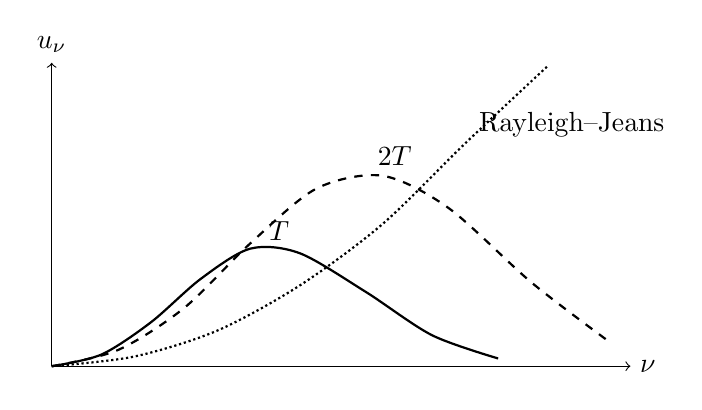
\begin{tikzpicture}[x=1.05cm,y=0.82cm]
\draw[->] (0,0)--(7.0,0) node[right] {\(\nu\)};
\draw[->] (0,0)--(0,4.7) node[above] {\(u_\nu\)};
\draw[densely dotted,thick] plot[smooth] coordinates
  {(0,0) (1,0.15) (2,0.55) (3,1.25) (4,2.20) (5,3.45) (6,4.65)};
\draw[thick] plot[smooth] coordinates
  {(0,0) (0.6,0.18) (1.2,0.68) (1.8,1.35) (2.4,1.82) (3.0,1.75) (3.8,1.15) (4.6,0.48) (5.4,0.12)};
\draw[thick,dashed] plot[smooth] coordinates
  {(0,0) (0.8,0.25) (1.6,0.90) (2.4,1.90) (3.2,2.75) (4.0,2.95) (4.8,2.45) (5.8,1.30) (6.7,0.42)};
\node[anchor=west] at (5.05,3.75) {Rayleigh--Jeans};
\node at (2.75,2.10) {\(T\)};
\node at (4.15,3.25) {\(2T\)};
\end{tikzpicture}
\caption{The classical spectrum rises without bound, while Planck spectra turn over. Increasing the temperature shifts the characteristic frequency upward and preserves the dimensionless shape.}
\label{fig:c07-planck-redraw}
\end{figure}

The overwhelming majority of photons in the present universe belong to the microwave background and have characteristic wavelength of order a millimeter. Equation~\eqref{eq:c07-thermal-wavelength} associates that wavelength with a few kelvin, conventionally rounded here to \(3\,\mathrm{K}\). A wavelength alone would provide only a rough association. The stronger evidence is that measurements over many frequencies trace the complete blackbody curve with very high precision.

\begin{classroomqa}
\audiencequestion{How much space does one microwave-background photon occupy?}
\lecturerresponse{A photon has no universal hard-edged size. It may be prepared as a wave packet whose spatial spread depends on the state, while its wavelength sets the scale of its oscillation. For the thermal background, both the characteristic wavelength and a natural wave-packet scale are of order a millimeter, but neither should be mistaken for the radius of a little classical object. \lecturetimestamp{00:57:16--00:59:05}}
\end{classroomqa}

\section{Expansion Freezes the Blackbody Shape}

Begin with a hot box containing ionized hydrogen and radiation in equilibrium. As the box expands, its contents do work, the energy density falls, and the temperature decreases. Eventually electrons and protons remain bound as neutral atoms. The formation of atoms is called \emph{recombination}; the loss of efficient photon--matter scattering is called \emph{decoupling}. The two processes are closely related but name different physical events.

After decoupling, matter and radiation no longer share a common temperature. Yet the photon spectrum retains its Planck form. Every freely propagating wavelength is stretched by the same expansion factor,
\begin{equation}
\lambda\propto a,
\qquad
\nu\propto a^{-1}.
\end{equation}
Because the Planck curve depends on \(\nu/T\), this uniform redshift is equivalent to assigning the radiation a temperature
\begin{equation}
\boxed{T_\gamma\propto a^{-1}.}
\label{eq:c07-temperature-scaling}
\end{equation}
Thus expansion preserves the shape even without collisions continually rebuilding it. Matter follows its own later thermal history.

The observed microwave background is therefore a fossil equilibrium distribution. Its blackbody form was established while free charges scattered efficiently and was then carried forward by uniform cosmological redshift. Starlight, gamma rays, and other later sources exist, but they are numerically small beside the relic photon population and have identifiable astrophysical origins.

\begin{classroomqa}
\audiencequestion{How can radiation remain blackbody after it is no longer in equilibrium with matter?}
\lecturerresponse{Collisions are needed to create the equilibrium spectrum, but not to preserve it under perfectly uniform expansion. Multiplying every wavelength by the same factor maps one Planck spectrum into another with a lower temperature. The photons cease sharing matter's temperature while retaining a blackbody temperature of their own.}
\end{classroomqa}

\section{Why Recombination Happens So Late}

The wavelength today and the wavelength at decoupling are related by
\begin{equation}
\frac{\lambda_0}{\lambda_{\rm dec}}
=
\frac{a_0}{a_{\rm dec}}
=
\frac{T_{\rm dec}}{T_0}.
\label{eq:c07-decoupling-ratio}
\end{equation}
Decoupling is not mathematically instantaneous, but it is short enough compared with the subsequent history that one may assign it a characteristic scale factor and temperature. Here \(T_0\) means the CMB temperature, not the kinetic temperature of intergalactic matter.

Hydrogen's ground-state ionization energy is
\begin{equation}
\chi_H=13.6\,\mathrm{eV}.
\end{equation}
A first guess would set \(k_BT\sim\chi_H\), so that a typical photon can ionize an atom. That guess is much too high because a thermal spectrum contains a high-energy tail and the universe contains an enormous number of photons.

\begin{figure}[htbp]
\centering

\includegraphics[width=0.82\textwidth]{lecture_07_figure_03.png}
\caption{The board introduces the observed abundance ratio \(N_\gamma/N_e=10^8\) and the photon-energy symbol \(\epsilon\). Only the beginning of the exponential is visible; the completed Boltzmann factor follows from the spoken derivation.}
\label{fig:c07-boltzmann-board}
\lectureframe{01:06:10.631}
\end{figure}

The rounded abundance ratio used here is
\begin{equation}
\frac{N_\gamma}{N_e}\sim10^8.
\label{eq:c07-photon-electron-ratio}
\end{equation}
It is inferred by comparing the measured CMB photon density with the ordinary-matter inventory. For photon energy \(\epsilon\), the high-energy tail has Boltzmann form
\begin{equation}
P(\epsilon)\propto e^{-\epsilon/(k_BT)}.
\end{equation}
The number of ionizing photons available per atom is therefore estimated by
\begin{equation}
10^8 e^{-\chi_H/(k_BT)}.
\end{equation}
Ionization remains effective until this quantity falls to order unity.

Taking logarithms gives
\begin{equation}
\frac{\chi_H}{k_BT}
\sim
\ln 10^8
\simeq18.4,
\end{equation}
or, at the intended accuracy,
\begin{equation}
k_BT\sim\frac{\chi_H}{20}.
\label{eq:c07-tail-estimate}
\end{equation}
The characteristic photon can lie far below threshold because one ionizing photon from the tail is enough for each atom.

\begin{classroomqa}
\audiencequestion{Does the tail estimate count photons exactly at the threshold or all photons above it?}
\lecturerresponse{It counts photons at and above the threshold. Since the tail falls exponentially, most of that integral comes from energies near \(\chi_H\), so the simple exponential estimate captures the relevant order of magnitude. \lecturetimestamp{01:08:39--01:08:54}}
\end{classroomqa}

\begin{classroomqa}
\audiencequestion{Was the ratio \(N_\gamma/N_e\) also about \(10^8\) at decoupling?}
\lecturerresponse{To the approximation used here, yes. From decoupling back to substantially hotter epochs, expansion dilutes both populations by the same volume factor and does not create or destroy enough of either species to alter their ratio. At still higher temperatures, pair-production reactions require new bookkeeping. \lecturetimestamp{01:08:54--01:09:57}}
\end{classroomqa}

\begin{classroomqa}
\audiencequestion{Do photons emitted by stars contribute appreciably to this count?}
\lecturerresponse{No. Stars did not yet exist at recombination, and even today their photons are a tiny fraction of the CMB population. The ratio in equation~\eqref{eq:c07-photon-electron-ratio} concerns the relic thermal photons. \lecturetimestamp{01:11:44--01:12:39}}
\end{classroomqa}

\begin{classroomqa}
\audiencequestion{When electrons recombine with protons, should the emitted photons leave a sharp hydrogen feature in the blackbody spectrum?}
\lecturerresponse{While scattering and absorption remain fast compared with expansion, the radiation is continually reprocessed and remains close to thermal equilibrium. A sufficiently abrupt freeze-out could preserve a distortion, but slow near-equilibrium recombination prevents a large isolated line from replacing the blackbody form. \lecturetimestamp{01:12:42--01:14:07}}
\end{classroomqa}

The resulting classroom estimate is \(T_{\rm dec}\sim4\times10^3\,\mathrm{K}\). A direct conversion of \(\chi_H/20\) gives a somewhat higher number, leading to the suggestion that the effective denominator may be nearer \(40\). This is not a contradiction; it exposes the crudeness of replacing the full ionization balance by one tail count. A controlled equilibrium treatment uses the Saha relation,
\begin{equation}
\frac{x_e^2}{1-x_e}
=
\frac{1}{n_H}
\left(\frac{m_e k_BT}{2\pi\hbar^2}\right)^{3/2}
e^{-\chi_H/(k_BT)},
\label{eq:c07-saha}
\end{equation}
followed by nonequilibrium recombination kinetics. The rough argument is valuable because it identifies the dominant physics: the tiny baryon-to-photon ratio delays neutral-atom survival to a temperature far below \(\chi_H/k_B\).

\section{Redshift to the Surface of Last Scattering}

With \(T_0\simeq3\,\mathrm{K}\) and \(T_{\rm dec}\sim4\times10^3\,\mathrm{K}\), equation~\eqref{eq:c07-decoupling-ratio} gives
\begin{equation}
\boxed{
\frac{a_0}{a_{\rm dec}}
\sim
\frac{T_{\rm dec}}{T_0}
\sim10^3
}.
\label{eq:c07-decoupling-expansion}
\end{equation}
Equivalently, the last-scattering redshift is of order \(10^3\). Before this epoch the ionized plasma was opaque; after it, photons propagated nearly freely.

This thermal event occurred only a few hundred thousand years after the beginning of the hot expansion, conventionally quoted in the exchange as roughly \(380{,}000\) years. That interval is tiny beside the subsequent cosmic age. Since decoupling, lengths have grown by about \(10^3\) and comoving volume elements by about \(10^9\).

Decoupling is one thermal landmark, not the only event in the intervening history. Galaxy formation, star formation, and black-hole formation all occur later, but they are set aside here so that the thermal landmarks can be followed cleanly backward.

Looking outward is looking backward. Nearby shells show recent epochs; more distant shells show earlier ones. Our past light cone eventually meets the epoch of recombination, and its intersection with that epoch is the surface of last scattering. Earlier electromagnetic radiation repeatedly scattered from free charges and could not travel directly to us.

\begin{figure}[htbp]
\centering
\begin{coursefitfigure}
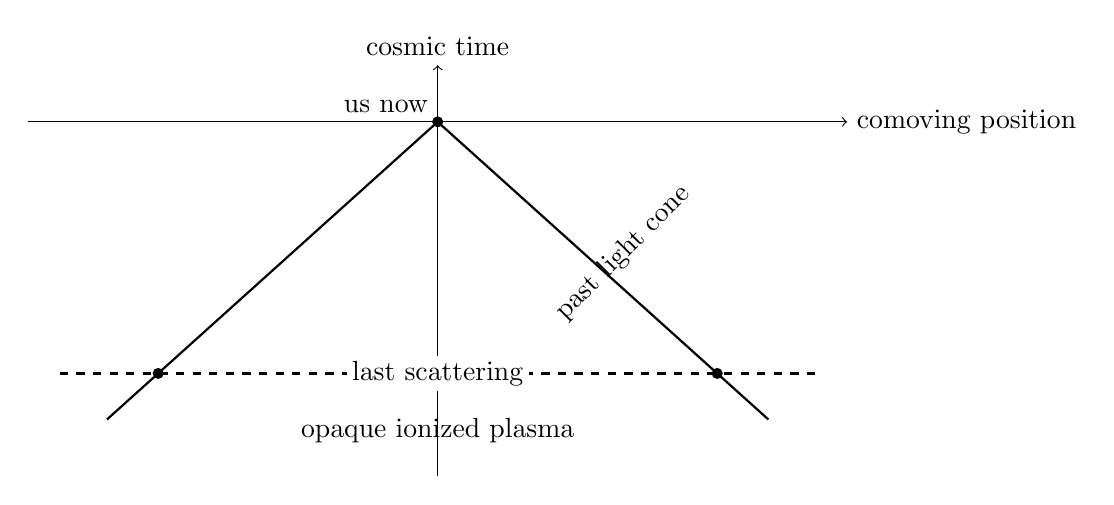
\begin{tikzpicture}[x=1.0cm,y=0.9cm]
\draw[->] (0,0)--(0,5.8) node[above] {cosmic time};
\draw[->] (-5.2,5.0)--(5.2,5.0) node[right] {comoving position};
\draw[thick] (0,5.0)--(-4.2,0.8);
\draw[thick] (0,5.0)--(4.2,0.8);
\draw[thick,dashed] (-4.8,1.45)--(4.8,1.45);
\fill (0,5.0) circle (2pt) node[above left] {us now};
\fill (-3.55,1.45) circle (2pt);
\fill (3.55,1.45) circle (2pt);
\node[fill=white,inner sep=2pt] at (0,1.45) {last scattering};
\node at (0,0.65) {opaque ionized plasma};
\node[rotate=45] at (2.35,3.15) {past light cone};
\end{tikzpicture}
\end{coursefitfigure}
\caption{Electromagnetic observation reaches back along the past light cone only to the last-scattering surface. Earlier photons were repeatedly scattered by the ionized plasma.}
\label{fig:c07-last-scattering}
\end{figure}

\begin{classroomqa}
\audiencequestion{Does decoupling end every possible observation of earlier epochs?}
\lecturerresponse{It ends direct electromagnetic viewing because the plasma was opaque to photons. More weakly interacting messengers could escape earlier: relic neutrinos in principle probe a deeper layer, and gravitational radiation could carry information from earlier still. Much of our knowledge beyond last scattering is therefore indirect but not arbitrary. \lecturetimestamp{01:32:27--01:36:31}}
\end{classroomqa}

\begin{classroomqa}
\audiencequestion{What was the absolute value of \(a\) at the beginning, and was the universe necessarily a tiny finite object?}
\lecturerresponse{In flat space only ratios of scale factors have invariant meaning; the normalization of \(a\) is arbitrary. A negatively curved spatial slice may also be infinite. A closed \(k=+1\) universe has a finite curvature radius, but observation still determines expansion ratios rather than a known primordial size. The hot big bang is not, by itself, the statement that all space was a tiny ball. \lecturetimestamp{01:30:05--01:32:22}}
\end{classroomqa}

\begin{classroomqa}
\audiencequestion{Because the CMB is older than galaxies, does seeing it tell us whether galaxies exist today beyond our observable region?}
\lecturerresponse{No. The CMB shows a distant region as it was at decoupling, not as it is today. Light from present-day galaxies at sufficiently great distance has not had time to reach us. What favors continued galaxy populations beyond our horizon is the observed large-scale homogeneity and the absence of a visible edge, not a direct view supplied by the CMB. \lecturetimestamp{01:59:01--02:00:58}}
\end{classroomqa}

The resulting timeline runs backward from the present through galaxy formation and decoupling to matter--radiation equality. Earlier still, the shrinking scale factor means increasing temperature and the appearance of new particle species.

\section{Matter--Radiation Equality}

Moving backward beyond decoupling, another landmark appears. Nonrelativistic matter and radiation dilute differently:
\begin{equation}
\rho_m\propto a^{-3},
\qquad
\rho_r\propto a^{-4},
\qquad
\frac{\rho_m}{\rho_r}\propto a.
\label{eq:c07-equality-scaling}
\end{equation}
Matter dominates late, but radiation inevitably dominates at sufficiently small \(a\). The expansion law changes correspondingly from the matter-era behavior \(a\propto t^{2/3}\) toward the radiation-era behavior \(a\propto t^{1/2}\).

A deliberately rough estimate starts with \(10^8\) photons per proton, characteristic CMB photon energy \(10^{-4}\,\mathrm{eV}\), and proton rest energy \(10^9\,\mathrm{eV}\). Ignoring dark matter gives
\begin{equation}
\left(\frac{\rho_m}{\rho_r}\right)_0
\sim
\frac{10^9}{10^8\,10^{-4}}
\sim10^5.
\end{equation}
The argument then corrects itself: dark matter contributes substantially more mass than luminous baryons, raising the rounded estimate to \(10^6\). Within this arithmetic, equation~\eqref{eq:c07-equality-scaling} places equality at
\begin{equation}
\frac{a_{\rm eq}}{a_0}\sim10^{-6},
\qquad
\frac{T_{\rm eq}}{T_0}\sim10^6.
\label{eq:c07-equality-estimate}
\end{equation}
These are scale-setting classroom estimates, not a precision cosmological parameter fit. Their purpose is to show how unequal powers of \(a\) locate successive thermal eras.

The radiation-dominated epoch lies behind the electromagnetic last-scattering wall, but its existence follows from the measured late-time densities and the known scaling laws. Continuing to higher temperature eventually invalidates the assumption that proton, electron, and photon numbers are separately fixed, because energetic collisions begin to create massive particle--antiparticle pairs.

\begin{classroomqa}
\audiencequestion{Does the statement that photon and proton numbers are conserved include starlight and arbitrarily high temperatures?}
\lecturerresponse{No. It applies to the relic CMB population over the interval in which number-changing reactions are ineffective. Starlight was created later and is negligible in the photon count. At sufficiently high temperature, pair creation changes the particle content and separate number conservation fails. Recombination itself adds at most roughly one photon per electron, only one part in \(10^8\) of the existing CMB population. \lecturetimestamp{01:26:24--01:27:40}}
\end{classroomqa}

\section{Pair Creation and the Almost Symmetric Soup}

At a temperature of order
\begin{equation}
T\sim10^{10}\,\mathrm{K},
\qquad
\frac{a_0}{a}\sim10^{14},
\end{equation}
the characteristic photon energy is around a mega-electron-volt, comparable to the rest-energy scale required to make an electron--positron pair. Two photons can then react through
\begin{equation}
\gamma+\gamma
\longleftrightarrow
e^-+e^+.
\label{eq:c07-pair-reaction}
\end{equation}
The exact threshold depends on collision kinematics, but the electron rest energy, \(m_ec^2\), sets the relevant scale.

Pair creation and annihilation rapidly balance one another. If too few pairs are present, photon collisions replenish them; if too many are present, annihilation returns their energy to photons. The abundances of photons, electrons, and positrons are therefore determined by temperature and are all of comparable order in the relativistic plasma. They no longer retain a simple memory of their later numbers.

\begin{classroomqa}
\audiencequestion{How can this pair-filled plasma remain electrically neutral if there are already electrons needed to balance protons?}
\lecturerresponse{Each reaction creates one negative and one positive charge, so the pairs add no net charge. They are an enormous nearly symmetric population superposed on a tiny electron excess. Individual electrons are indistinguishable; only the difference \(N_{e^-}-N_{e^+}\) remembers the charge needed to balance the protons. \lecturetimestamp{01:42:31--01:43:14}}
\end{classroomqa}

Pair reactions change the sum but preserve the difference:
\begin{equation}
N_{e^-}+N_{e^+}\quad\hbox{changes},
\qquad
N_{e^-}-N_{e^+}=\hbox{constant}.
\label{eq:c07-pair-invariants}
\end{equation}
In the hot soup \(N_{e^-}+N_{e^+}\) is of the same order as \(N_\gamma\), whereas the surviving excess is of the same order as the much smaller proton number. Hence the rounded ratio is
\begin{equation}
\boxed{
\frac{N_{e^-}-N_{e^+}}
{N_{e^-}+N_{e^+}}
\sim10^{-8}
}.
\label{eq:c07-asymmetry}
\end{equation}
There was roughly one excess electron for every \(10^8\) electron--positron pairs.

This reverses the original question. The striking fact is not simply that photons are numerous. At high temperature photons and pairs naturally have comparable abundances. The puzzle is why the negative and positive particle populations differ at all, and why their relative difference is tiny rather than exactly zero or of order unity. A symmetric initial state and symmetric pair production would give no excess. The microscopic origin of the nonzero asymmetry is the problem carried into the next stage of the discussion.

At temperatures another two or three orders of magnitude higher, proton structure can no longer be ignored. Collisions produce quarks and antiquarks, while protons dissolve into their constituents; photons, leptons, quarks, antiquarks, gluons, and whatever dark species are light enough form a hotter plasma. Vacuum energy is dynamically negligible there because radiation density grows as \(a^{-4}\).

The corresponding quark excess is tied to the electron excess by overall charge neutrality. Three valence quarks make a baryon, so the bookkeeping differs by conventional factors, but the surviving baryonic matter and the surviving electrons are not independent charge imbalances. Their common smallness is a relic of the early universe.

Follow the electron--positron plasma forward again. Once the temperature falls below the pair-production scale, annihilation continues while the reverse reaction becomes rare. Almost every electron finds a positron, the pair energy becomes radiation, and only the tiny unmatched electron population remains. The matter around us is this residual imbalance, not a representative sample of the once enormous pair population.

\begin{classroomqa}
\audiencequestion{What were the protons doing during the electron--positron annihilation era?}
\lecturerresponse{At that stage the temperature was high enough to create electron pairs but not yet high enough to create abundant proton--antiproton pairs or dissolve protons into quarks. The proton population was therefore small but persistent, and neutrality required \(N_{e^-}-N_{e^+}\simeq N_p\). \lecturetimestamp{01:55:35--01:56:53}}
\end{classroomqa}

The visible universe appears to have the same sign of matter excess throughout. The classroom evidence offered is the absence of antinuclei in cosmic rays: secondary collisions can make occasional antiprotons, but an antigalaxy would be expected to supply complex antinuclei. This is a lecture-era observational argument and not a claim that regions beyond the observable horizon have been inspected.

\begin{classroomqa}
\audiencequestion{Could the observed matter excess be a local fluctuation, with antimatter regions beyond what we can see?}
\lecturerresponse{The same sign across the enormous observable volume is far too coherent to be a random fluctuation. It demands a dynamical explanation. Beyond the observable region, however, direct evidence is unavailable; a transition to a different domain cannot be ruled out merely by looking farther than light has reached us. \lecturetimestamp{01:56:57--01:58:47}}
\end{classroomqa}

\begin{classroomqa}
\audiencequestion{Is the matter--antimatter explanation already a precise numerical theory, and does force unification occur at this temperature?}
\lecturerresponse{There is a qualitative theory of how a small asymmetry can arise, but the rounded \(10^{-8}\) value is not derived here from a unique microscopic model. Force unification belongs to temperatures much higher than the electron-pair epoch. Both questions require physics beyond the present thermal landmarks. \lecturetimestamp{01:51:36--01:52:24}}
\end{classroomqa}

\section{What to Carry Forward}

The thermal history is organized by rates and thresholds. Rapid scattering gives a common temperature; neutral-atom formation removes the scatterers; uniform expansion then redshifts a frozen Planck spectrum without destroying its shape. The CMB is therefore both a thermometer for the radiation and a visible surface marking the end of direct electromagnetic access to the earlier plasma.

The photon excess makes recombination a tail problem rather than an average-energy problem. The scale \(T_{\rm dec}/T_0\sim10^3\) locates last scattering, while the unequal dilution laws for matter and radiation locate an earlier equality era. At still higher temperature, pair creation erases memory of the total electron and positron numbers but preserves their tiny difference. That residual asymmetry, mirrored in the baryonic sector, is the unexplained initial datum that the next investigation must confront.
